\documentclass[12pt, a4paper, openany]{book}
\usepackage[italian]{babel}
\usepackage{listings}
\usepackage{graphicx}
\usepackage{fancyvrb}
\graphicspath{ {./images/} }

\begin{document}

\title{Basi di dati}
\author{Fabio Ferrario}
\date{Gennaio 2022}

\maketitle
\tableofcontents


\chapter{Schema Entity-Relationship}

\section{Introduzione}
Lo schema ER, o Entity Relationship, è un modello intermedio per la produzione di un Database che serve a rappresentare in modo semplice e comprensibile la struttura di una base di dati.
\\Lo schema ER è un modello concettuale che rappresenta solo lo "schema", quindi la struttura, del database ma non può rappresentarne le istanze ed è indipendente da ogni DBMS.
\\Uno schema ER è formato da vari costrutti che rappresentano l'intera struttura della base di dati.

\section{I costrutti di ER}
Come detto in precedenza ER ha molti costrutti che vengono rappresentati in maniera varia, che però possiamo generalizzare come in figura:
\\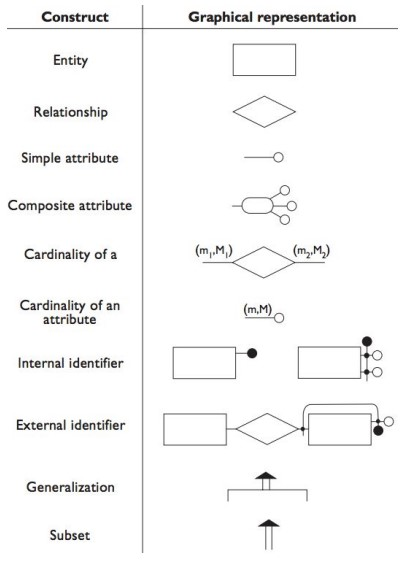
\includegraphics{rappresentazione-er.jpg}
\\Di seguito elenchiamo i vari costrutti.
\subsection{Entità}
Un'entità è una classe di oggetti con proprietà comuni ed esistenza autonoma della quale si registrano
fatti specifici.

\paragraph{Nome} Ogni entità ha un nome univoco, espressivo e al \textbf{singolare}.

\paragraph{Rappresentazione} Sono rappresentate da un rettangolo con all'interno il nome dell'entità.

\paragraph{Caratteristiche} Ogni entità ha vari attributi, di (almeno) uno è necessariamente identificatore (chiave primaria).

\subsection{Relazione}
Una relazione descrive un'azione o una situazione e stabilisce legami logici tra istanze di entità; possono essere tra più di due entità e il numero di esse coinvolte determina il grado della relazione, che può essere binaria, ternaria o n-aria.

\paragraph{Nome} Una relazione è identificata univocamente da un sostantivo.

\paragraph{Rapresentazione} Vengono appresentate da un rombo con all'interno il nome della relazione, è collegato alle entità da dei connettori con indicata la cardinalità della relazione.

\paragraph{Caratteristiche} Una relazione zero o più attributi ma NON ha identificatori.

\subsection{Attributi}
Gli attributi associano ad ogni istanza di entità o relazione un valore, definito su un dominio di valori, specificato nella documentazione associata, con il fine di descrivere le proprietà elementari di entità/relazioni disegnate per rappresentare la realtà di interesse
\subsubsection*{Attributo semplice}
Un attributo è semplice se è formato da un solo elemento (attributo).
\paragraph{Rappresentazione} Sono rappresentate da un'asticella con un pallino ad una estremità

\subsubsection*{Attributo composto}
Raggruppamento di attributi di una medesima entità/relazione con affinità di significato e/o uso.

\subsection{Cardinalità delle relazioni}
Vengono specificate per ogni relazione e descrivono il numero minimo e massimo di occorrenza di relazione, a cui una occorrenza dell'entità può partecipare alla relazione, ossia quante volte un'occorrenza di un'entità può essere legata ad occorrenza delle altre entità coinvolte.
\\è possibile assegnare alla cardinalità un qualunque intero non negativo, con l'unico vincolo che la cardinalità minima sia minore o uguale alla cardinalità massima e di solito si usano i valori 0, 1 e N.

\subsection{Cardinalità di un attributo}
Descrive il numero minimo e massimo di valori dell'attributo associati all'entità e/o relazione, con la cardinalità (1,1) stabilità come default, che può essere vista come funzione che associa ad ogni occorrenza di entità un solo valore dell'attributo; si hanno le stesse consuetudini delle cardinalità delle relazioni.

\subsection{Identificatori}
Gli identificatori sono attributi che permettono di identificare in maniera univoca un'entità. Possono essere interni ed esterni e formati da un'attributo, un gruppo di attributi o un insieme di più attributi separati
\subsubsection{Identificatore Interno} 
Un identificatore è interno in caso sia uno più attributi dell'entità stessa che identificano, tutti con cardinalità (1,1)

\subsubsection{Identificatore Esterno}
Un identificatore è esterno se è un attributo di un entità diversa da quella che identifica, in cui esiste una relazione uno a uno tra le due entità.

\subsection{Generalizzazione}
Anche dette Is-a, una generalizzazione è un'entità che eredita tutti gli attributi e le relazioni di un'altra entità
(detta padre), rappresentata da una freccia (ramata) che va dai figli verso il padre.
\paragraph*{Generalizzazione Totale}
Una generalizzazione viene detta totale se ogni occorrenza del genitore è un'occorrenza di almeno uno dei figli, altrimenti è parziale

\paragraph*{Sottoinsieme}
è una generalizzazione con soltanto un entità figlia, di cui solitamente rappresenta una parte dell'entità genitore.

\section{Qualità degli schemi ER}
Come già detto, uno schema ER deve rappresentare completamente la struttura di una base di dati, e deve farlo in modo efficiente e comprensibile. Una determinata richiesta per una base di dati può essere soddisfatta da più schemi ER, alcuni però lo fanno meglio di altri.
\\Quindi possiamo definire alcuni indicatori della qualità degli schemi ER:
\begin{itemize}
    \item Correttezza rispetto al modello
    \item Correttezza rispetto ai requisiti
    \item Minimalità (e ridondanza)
    \item Competenza e pertinenza
    \item Leggibilità grafica
    \item Compattezza
\end{itemize}
\chapter{Modello Relazionale}

\section{Introduzione}
Dove lo schema ER è un modello concettuale per rappresentare una base di dati, il Modello Relazionale è il \textbf{Modello Logico} necessario per rappresentare in maniera efficace ed efficiente la base dati modellata.
Il modello relazionale è utilizzato in molti DBMS, e in esso ogni tabella è formata da Relation Schema e Relation Instance.
Questo modello presenta una notevole differenza da ER, dato che i riferimenti fra dati in strutture diverse sono rappresentati per mezzo dei valori stessi, garantendo così l'indipendenza dei dati.

\paragraph{Relation Schema e Relation Instance}
Nel modello relazionale ogni relazione può essere rappresentata in due modi, lo schema e l'istanza.
\\Lo \textbf{schema di una relazione} è invariante nel tempo e descrive la struttura, quindi l'aspetto intensionale della relazione. Viene rappresentato con il nome della tabella e l'elenco degli attributi.
\\L'\textbf{istanza di una relazione} invece sono i valori effettivi della relazione che possono cambiare nel tempo (aspetto estensionale). Viene rappresentato come la tabella della relazione con le isanze.


\section{I vincoli di integrità}
Una relazione è una rappresentazione di un frammento di realtà osservata, quindi possono esistere istanze di basi di dati che, pur sintatticamente corrette, non rappresentano stati possibili nella realtà.
\\Introduciamo quindi il concetto di vincolo di integrità, una proprietà che deve essere soddisfatta da tutte le istanze di uno schema che rappresentano informazioni corrette per l'applicazione
\subsection{Vincoli intrarelazionali}

\paragraph*{Vincoli di Tupla}
I vincoli che vengono valutati su una sola Tupla di una relazione sono detti vincoli di tupla, e vengono espressi con sintassi booleana.
\\Se questo vincolo viene valutato su più attributi di una sola tupla, quindi limita il valore di un attributo in base al valore di un altro attributo della stessa ennupla, allora è detto vincolo di \textbf{Tupla}.
\\Se un vincolo di tupla è valutato su un singolo attributo è detto di \textbf{Dominio}, che quindi limita il dominio di quel singolo attributo (per esempio voto < 30)


\paragraph*{Vincolo di Relazione}
Vincolo relativo all'insieme di Ennuple di una relazione

\paragraph*{Vincolo di Chiave}
Vincolo che permette di avere la certezza dell'inicità di uno schema di relazione. I vincoli di chiave nascono dalla necessità di individuare informazioni che ci permettano di rappresentare ogni oggetto di interesse con una ennupla differente e identificarlo quando se ne abbia necessità.
\\Una \textbf{Superchiave} è un insieme di attributi che identificano le ennuple di una relazione, quindi è un insieme di attributi per cui nella relazione non possono esistere due tuple che hanno gli stessi valori degli attributi contenuti nella superchiave.
\\Se una superchiave non contiene propriamente un'altra superchiave, viene detta \textbf{Chiave} oppure \textbf{Superchiave Minimale}

\chapter{Progettazione Logica}
\section{Introduzione}
L'obiettivo della progettazione logica è quello di costruire uno schema logico in grado di descrivere, in maniera corretta ed efficiente, tutte le informazioni contenute nello schema ER prodotto nella fase di progettazione concettuale.
Nella Progettazione Logica si hanno due necessità:
\begin{itemize}
    \item Semplificare la traduzione
    \item Ottimizzare il progetto
\end{itemize}
La semplificazione dello schema si rende necessaria perchè \emph{non tutti i costrutti del modello ER hanno una traduzione naturale nei modelli logici}, vedisi la generalizzazione.
\\Inoltre, mentre la progettazione concettuale ha come obiettivo la rappresentazione accurata e naturale dei dati dal punto di vista del significato che hanno nell'applicazione, quindi in modo da renderli comprensibili nel mondo reale, 
\textbf{la progettazione logica costituisce la base per l'effettiva realizzazione dell'applicazione}
e deve tenere conto, per quanto possibile, delle sue prestazioni: questa necessità può portare a una ristrutturazione dello schema concettuale che renda più \emph{efficiente} l'esecuzione delle operazioni previste.
\\Pertanto è necessario prevedere sia a un'attività di \textbf{riorganizzazione} del modello concettuale, sia un'attività di \textbf{traduzione} da concettuale a logico.


\section{Ristrutturazione di ER}
Come già detto, la progettazione logica prevede una parte di riorganizzazione (ristrutturazione) dello schema ER.
\\Questa fase si può suddividere in una serie di passi da effettuare in sequenza:
\begin{enumerate}
    \item \textbf{Analisi delle ridondanze}, dove si decide se eliminare o mantenere eventuali ridondanze presenti nello schema
    \item \textbf{Eliminazione delle generalizzazioni}, dove tutte le generalizzazioni presenti nello schema vengono analizzate e sostituite da altri costrutti
    \item \textbf{Partizionamento o accorpamento} di entità e associazioni, dove si decide se è opportuno partizionare concetti dello schema (entità e/o associazioni) in più concetti o, viceversa, accorpare concetti separati in un unico concetto
    \item \textbf{Scelta degli identificatori principali}, dove si seleziona un identificatore per quelle entità che ne hanno più di uno
\end{enumerate}
\subsection{Analisi delle ridondanze}
Un attributo ridondante è un attributo che può essere derivato da altri attributi. Ci sono varie forme di ridondanza ma riportiamo alcuni casi frequenti:
\begin{itemize}
    \item Attributi derivabili, occorrenza per occorrenza, da altri attributi della stessa entità o associazione
    \item Attributi derivabili da attributi di altre entità (o associazioni), di solito attraverso funzioni aggregative.

\end{itemize}
In generale la presenza di un dato derivato presenta un vantaggio e alcuni svantaggi, quindi la decisione di mantenere o eliminare una ridondanza va presa confrontando costo di esecuzione delle operazioni che coinvolgono il dato ridondante e la relativa occupazione di memoria.
\subsection{Eliminazione delle Generalizzazioni}
Le generalizzazioni non sono rappresentabili nel Modello Relazionale, quindi è compito della Progettazione Logica di eliminarle mantenendo la correttezza dello schema.\\
Per fare questo ci sono tre modi:
\subsubsection{Accorpamento dei figli nel genitore} Viene usato quando l'accesso alle entità è contestuale
\\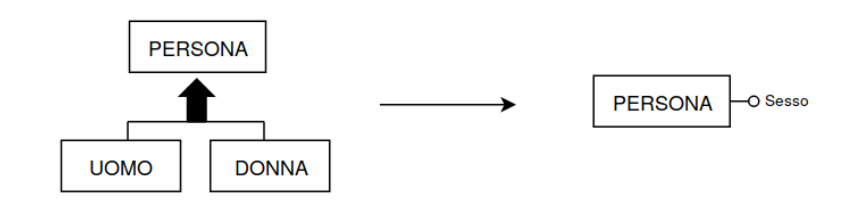
\includegraphics[width=\textwidth]{generalizzazioni1.png}
\subsubsection{Accorpamento del genitore nei figli}
Possibile solo se la generalizzazione è totale
\\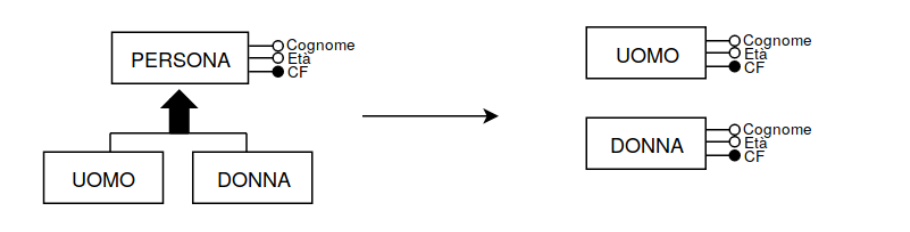
\includegraphics[width=\textwidth]{generalizzazioni2.png}
\subsubsection{Sostituzione di generalizzazione con associazioni}
Si usa quando l'accesso alle due entità è separato. Conveniente con generalizzazione parziale
\\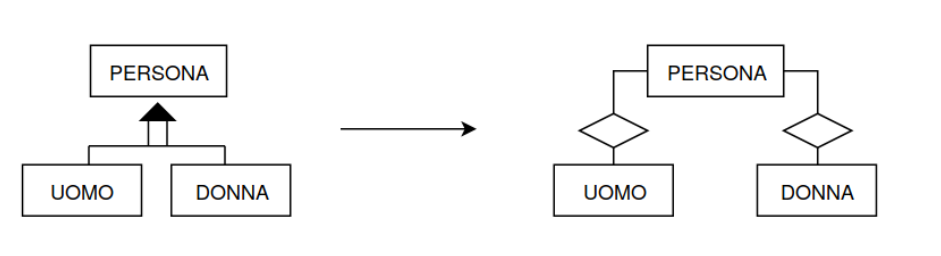
\includegraphics[width=\textwidth]{generalizzazioni3.png}

\chapter{Algebra Relazionale}
\section{Introduzione}
L'algebra relazionale è un linguaggio per basi di dati di tipo Procedurale.
\\
AR è un linguaggio prettamente formale che forma la base per linguaggi 'reali'. è di tipo procedurale, quindi viene specificato l'algoritmo con cui ottenere il risultato. In AR istruzioni equivalenti
possono differire in termini di efficienza.\\
Le relazioni vengono intese in senso matematico, quindi insieme di tuple definite su attributi. In un insieme non ci possono essere elementi uguali. 

\section{Gli operatori di AR}
L'algebra relazionale ha 7 operatori che danno l'intero potere espressivo del linguaggio e grazie a una combinazione di questi è possibile interrogare la base di dati

\begin{itemize}
    \item Operatori insiemistici
    \subitem $\cup$ Unione 
    \subitem $\cap$ Intersezione 
    \subitem $-$ Differenza
    \item $\rho$ Ridenominazione
    \item $\sqcap$ Proiezione
    \item $\sigma$ Selezione
    \item $\bowtie$ Join

\end{itemize}
il Join lo considereremo come un operatore "a parte"

\subsection{Operatori insiemistici}
Una relazione (in matematica) è un sottoinsieme del prodotto cartesiano di due o più insiemi.
Una relazione è un insieme, quindi: non c'è ordinamento tra le tuple, ogni tupla è distinta e al suo interno è ordinata.
\\ Visto che le relazioni sono insiemi, è possibile applicare operatori tra insiemi che producono insiemi.
\\Nota bene: Le operazioni di Unione, Intersezione e differenza sono applicabili solo a relazioni definite sugli stessi attributi.
Visto che i risultati devono essere relazioni, le n-ple identiche nel risultato vengono unite in una unica n-pla.
\subsubsection*{Unione}
\begin{lstlisting}[mathescape=true]
$r_1 \cup r_2$
\end{lstlisting}
Produce tutte le n-ple delle relazioni $r_1$ e $r_2$
\\L'unione è commutativa e associativa
\subsubsection*{Intersezione}
\begin{lstlisting}[mathescape=true]
$r_1 \cap r_2$
\end{lstlisting}
Produce tutte le n-ple che appartengono sia a $r_1$ che $r_2$
\\L'intersezione è commutativa e associativa
\subsubsection*{Differenza}
\begin{lstlisting}[mathescape=true]
$r_1 - r_2$ 
\end{lstlisting}
Produce tutte le n-ple di $r_1$ che non compaiono anche in $r_2$
\\La differenza non è ne commutativa, ne associativa

\subsection{$\rho$ Ridenominazione}
\begin{lstlisting}[mathescape=true]
$\rho_{y \leftarrow x} (r)$
\end{lstlisting}
Cambia il nome dell'attributo $x$ della relazione $r$ in $y$
\\ATTENZIONE: la ridenominazione modifica lo schema lasciando inalterata l'istanza di r
\\è possibile rinominare più attributi contemporaneamente usando $\rho_{y,z \leftarrow x,w} (r)$
\\\textbf{REMEMBER} la ridenominazione è in ordine $nuovoNome \leftarrow vecchioNome$ 

\subsection{$\sqcap$ Proiezione}
\begin{lstlisting}[mathescape=true]
$\sqcap_{listaAttributi}(r)$
\end{lstlisting}
La proiezione "decompone verticalmente" la tabella, riportando solo gli attributi contenuti in listaAttributi di tutte le n-ple.
\\Gli attributi in listaAttributi sono separati da una virgola

\subsection{$\sigma$ Selezione}
\begin{lstlisting}[mathescape=true]
$\sigma_{condizione}(r)$
\end{lstlisting}
La selezione è un operatore ortogonale alla proiezione, quindi "decompone orizzontalmente" una tabella. Produce una relazione che ha lo stesso schema dell'operando e contiene un sottoinsieme delle ennuple dell'operando, quelle che soddisfano la condizione espressa dall'operatore
\paragraph{Condizione}
La condizione è una espressione booleana ottenuta combinando con i connettivi OR, AND e NOT condizioni atomiche. Le condizioni atomiche sono del tipo confronto tra attributi o tra un attributo e una costante
\section{$\bowtie$ Join}
Il join è un operatore fondamentale dell'AR che ci permette di combinare tuple appartenenti a relazioni diverse. Il Join produce il sottoinsieme del prodotto cartesiano di due relazioni in cui il valore di determinati attributi coincide
\subsection*{Varianti del join}
\begin{itemize}
    \item Join Naturale
    \item Prodotto cartesiano
    \item Theta Join
    \item Join esterno (Destro e Sinistro)
\end{itemize}
\subsection{Join Naturale}
\begin{lstlisting}[mathescape=true]
$r_1(X_1) \bowtie r_2(X_2)$
\end{lstlisting}
Il Join Naturale combina le tuple delle due relazioni sulla base dell'uguaglianza dei valori degli attributi comuni, quindi se faccio il join di due relazioni cercherà una corrispondenza tra gli attributi con lo stesso nome e produrrà una tupla corrispondente.
\\Date due relazioni r1 e r2, ogni tupla che compare nel risultato del join naturale è ottenuta come combinazione di una tupla di r1 con una di r2 sulla base dell'uguaglianza dei valori degli attributi comuni alle due relazioni.\\
Lo schema del risultato è l'unione degli schemi degli operandi $X1 \cup X2$
\\Quando una tupla non partecipa al risultato (per esempio un valore appare in una tabella ma non nel risultato) viene detto Dangling e il Join diventa incompleto
\\Se due relazioni sono definite sugli stessi attributi il join naturale equivale all'intersezione delle due relazioni
\paragraph{Attenzione} se facciamo il join naturale di due relazioni che non hanno attributi comuni (con lo stesso nome) il risultato sarà il prodotto cartesiano delle due! 

\subsection{Theta Join}
\begin{lstlisting}[mathescape=true]
$r_1(X_1) \bowtie_{condizione}$ $r_2(X_2)$
\end{lstlisting}
Succede spesso che due relazioni non hanno attributi comuni, quindi il join genererebbe il prodotto cartesiano che ha senso solo se è seguito da una selezione.
\\Il theta join effettua un Join con una immediata selezione, di modo da dar senso al prodotto cartesiano.
\paragraph{Attenzione} Il theta join si applica SOLO quando $X_1$ e $X_2$ sono insiemi disgiunti, altrimenti un join normale sarebbe sufficiente.

\subsection{Join Esterno}
\begin{lstlisting}[mathescape=true]
$r_1$ JOIN$_{LEFT/RIGHT/FULL}$ $r_2$
\end{lstlisting}
Il join esterno è un tipo di join naturale che mantiene tutte le tuple di uno o entrambi gli operandi, estendendo le tuple che rimarrebbero dangling con dei valori nulli, eliminando quindi il tuple dangling
Quando facciamo un join naturale stiamo facendo un join interno, quindi se esistono delle tuple che non appartengono al risultato rimangono dangling.
\\In caso volessimo mantenere tutte le tuple di una o entrambe le operazioni, usiamo il join esterno.
\paragraph{Tipi di join esterno}
\begin{itemize}
    \item LEFT, che mantiene tutte le tuple del primo operando
    \item RIGHT, che mantiene tutte le tuple del secondo operando
    \item FULL, che mantiene tutte le tuple di entrambi gli operandi
\end{itemize}

\subsection{Self Join}
In alcuni casi bisogna fare un join di una relazione con (una copia di) se stessa, chiamiamo questo tipo di Join "self join".
\\Generalmente viene usato per:
\begin{itemize}
    \item Confrontare tuple di una relazione tra loro
    \item trovare elementi duplicati
    \item Quando una tuple fa riferimento a dati della stessa tabella
\end{itemize}
Un modo per fare un self join è (per esempio) un join tra una relazione (con opportuno select etc) e una proiezione di un attributo di se stessa

\section{Gestione dei valori NULL}
Nelle basi di dati possiamo incontrare dei valori nulli, quindi AR utilizza una logica a tre valori: True, False e NULL.
\\In generale l'introduzione di un NULL nella logica classica non varia il risultato, tranne in due casi:
\begin{itemize}
    \item NULL AND True -> NULL
    \item NULL OR False -> NULL
\end{itemize}

\subsection*{condizione IS NULL}
Quando si necessita una condizione si possono usare IS NULL e IS NOT NULL, che diventano true rispettivamente se il dato è Nullo e se non è Nullo

\section{Le Viste}
Per semplificare alcune espressioni è utile avere delle relazioni derivate a partire dalle relazioni definite nello schema di base di dati.
\\é quindi possibile in AR definire delle viste, che altro non sono che delle espressioni a cui viene assegnato un nome che possono essere usate all'interno di altre espressioni

\begin{lstlisting}
nome_vista = ESPRESSIONE AR
\end{lstlisting}

\paragraph{Attenzione} Le viste sono relazioni virtuali, quindi non vengono mai salvate nella base di dati, quindi una interrogazione su una vista viene eseguita "ricalcolando" la vista


\section{Produrre interrogazioni in AR}
Esiste un metodo "generale" per produrre interrogazioni in algebra relazionale:
\begin{enumerate}
    \item Dalla "domanda" trova l'insieme di relazioni su cui applicare gli operatori
    \item Procedi secondo la strategia "dall'interno all'esterno"
\end{enumerate}
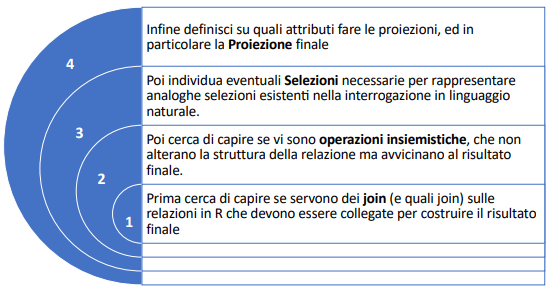
\includegraphics{AR1.png}
\paragraph{In parole povere}
Per produrre con efficienza delle interrogazioni i AR bisogna procedere a strati, partendo da quello più interno (il Join) e finendo con la proiezione degli attributi

\section{Esercizi}
Dato il seguente schema relazionale:
\begin{lstlisting}
Personale_non_docente(Matricola_d,Cognome,Nome, Ruolo, Classe_stipendio)
Personale_docente(Matricola_d,Cognome,Nome,Ruolo, Classe_stipendio)
Stipendio(Classe,Valore)

Studente(matricola_st,Cognome,Nome, corso_di_Laurea)

\end{lstlisting}
\paragraph{es16} Formulare l'espressione in AR che produca le classi di stipendio che non sono attribuite a nessun personale docente - senza usare l'operatore differenza
\begin{lstlisting}[mathescape=true]
PROJ$_{classe_stipendio}$(
    SEL$_{matricola_d IS NULL}$(
        personale_docente $\bowtie_{RIGHT JOIN}$ RID$_{classe\_stipendio \leftarrow classe}$(stipendio)
    )
)
\end{lstlisting}
\paragraph*{Note su es16}
la rinominazione di "classe\_stipendio" in "classe" può essere evitata facendo un THETA RIGHT JOIN,
quindi con $ \bowtie_{RIGHT classe = classestipendio} $


\paragraph*{es17}Formulare una espressione in AR che produca il personale non docente che è anche iscritto ad un corso di laurea senza usare l'operatore intersezione o differenza
\begin{lstlisting}[mathescape=true]
    PROJ$_{matricola\_d,Cognome\_nome}$(
        PROJ$_{matricola\_st,cognome,nome}$(personale\_non\_docente)
        JOIN$_{matricola\_d = matricola\_st}$
        PROJ$_{matricola\_st,cognome,nome}$(studente) 
    )   
\end{lstlisting}
\paragraph*{Note su es17}
La prima proiezione serve a eliminare il doppione "matricola\_s" che verrebbe generato dal join\\
Le due piccole proiezioni invece servono a eliminare gli attributi non comuni perchè il join in AR va sempre fatto tra relazioni con gli stessi attributi
\chapter{SQL}
\section{Introduzione}
SQL è il linguaggio per la definizione e la manipolazione dei dati in database relazionali adottato da tutti i principali DBMS.\\
Nonostante sia uno standard solo parte dei DMBS lo utilizza, ed esistono tre livelli di conformità che differiscono a seconda delle features implementate:
\begin{itemize}
    \item Entry
    \item Intermediate
    \item Full
\end{itemize}
La maggior parte dei database è conforme all'Entry, ma Intermidiate è la versione che più soddisfa le esigenze di mercato
\subsection*{SQL e AR}
SQL è "relazionalmente completo", quindi ogni espressione di AR può essere tradotta in SQL, però quest'ultimo può fare molto di più.
\\Come AR SQL adotta una logica a tre valori (T,F,?), e la gestione dei valori NULL è la medesima. Inoltre SQL è un linguaggio computazionalmente completo.
A differenza di AR in SQL le relazioni sono intese come tabelle e possono esserci righe uguali
\subsection*{Funzionalità}
SQL estende molto AR, in particolare contiene:
\begin{itemize}
    \item DDL(Data definition language)
    \subitem Operazioni di definizione e modifica dello schema
    \item DML(Data Manipulation Language)
    \subitem Operazioni di interrogazione
    \subitem Operazioni di Aggiornamento 
\end{itemize}
\section{SQL-DDL}
SQL-DDL, o data definition language è la parte di SQL che ti permette di effettuare operazioni di definizione e modifca degli schemi di una base di dati.
Con SQL-DDL si possono descrivere tre aspetti di uno schema relazionale: Schema, Table e Domain.
\subsection{L'istruzione CREATE TABLE}
\begin{lstlisting}
CREATE TABLE TableName
(AttributeName Domain [DefaultValue] [Constraints]
,...,
[OtherConstraints])
\end{lstlisting}
L'istruzione CREATE TABLE definisce uno schema di relazione e ne crea un'istanza vuota, cioè senza ennuple, di cui specifica attributi, domini e vincoli

\paragraph{Domini o data types}
esistono due tipi di domini: elmentari e definiti dall'utente.
\\Tra i domini elementari troviamo: Testuali, Numerici, Data e ora, Booleani, BLOB e CLOB.
\\I domini definiti dall'utente invece sono creati dall'istruzione CREATE DOMAIN che definisce un dominio elementare utilizzabile in definizioni di relazioni, anche con vincoli e valori di default
\subsubsection{Vincoli}
SQL-DDL può anche definire i vincoli di integrità intra-relazionali e inter-relazionali.
\paragraph{Vincoli Intrarelazionali} 
Definiti tramite: NOT NULL, UNIQUE, PRIMARY KEY, CHECK

\paragraph{Vincoli Interrelazionali} FOREIGN KEY e REFERENCES, che sono vincoli di integrità referenziale

\section{Istruzione SELECT}
In SQL ogni query di interrogazione inizia con l'istruzione SELECT che select non ha niente (circa) a che fare con la selezione di AR. Il risultato di una SELECT è sempre una tabella e una tabella è sempre ottenuta tramite una Select.
\\Nella sua forma più base
\begin{lstlisting}
SELECT listaAttributi <-- target list
FROM tabella
[WHERE condizione]
\end{lstlisting}
Seleziona tra le n-ple del prodotto cartesiano delle tabelle citate nella
FROM, quelle che soddisfano la condizione presente nella WHERE, e di
esse ne rappresenta solo gli attributi nella ListaAttributi.
\subsection{Le clausole e condizioni di Select}
L'istruzione select ha moltissime possibili clasuole o condizioni che modificano o estendo il risultato di una query.

\subsection*{SELECT DISTINCT} 
In generale, in una query SELECT i duplicati vengono mantenuti. \emph{Se Si vogliono eliminare i duplicati} si può usare l'istruzione SELECT DISTINCT.
\begin{verbatim}
    SELECT DISTINCT attributo1, attributo2, ...
\end{verbatim}
La clausola distinct elimina i duplicati \emph{considerando tutta la ennupla e non solo un singolo attributo}.
\subparagraph{Attenzione} DISTINCT da solo non esiste, se si usa va sempre indicato come SELECT DISTINCT

\subsection*{AS}
La clausola AS serve a rinominare gli attributi in modo da semplificarne la comprensione o velocizzare la scrittura
\begin{verbatim}
    SELECT attributo1 AS nuovonome, attributo2 AS ...
\end{verbatim}

\paragraph*{} AS può anche essere utilizzato per rinominare le tabelle, però può anche essere omesso. Quindi:
\begin{verbatim}
    SELECT ...
    FROM tabella AS T
\end{verbatim}
equivale a dire
\begin{verbatim}
    SELECT ...
    FROM tabella T
\end{verbatim}

\subsection*{Clausola . (punto)}
Quando nella SELECT si considerano più tabelle (con un JOIN o un prodotto cartesiano) si potrebbe aver bisogno di specificare a quale tabella appartiene l'attributo che si sta considerando per una condizione (quindi in WHERE o HAVING).
Per fare ciò si può usare la clausola \textbf{.} (punto), sia in caso la tabella è stata rinominata sia in caso contrario.

\begin{verbatim}
    SELECT ...
    FROM tabella T
    WHERE T.attributo1 ...
\end{verbatim}

\subsection*{Aritmetica nella target list}
La SELECT ci permette di utilizzare degli operatori aritmetici nella targetl list.\\
gli operatori aritmetici consentiti sono i classici +, -, *, / e la priorità è quella standard e alterabile con delle parentesi.
\begin{verbatim}
    SELECT attr1 + attr2
    FROM ...
\end{verbatim}
Questa query produrrà una tabella che avrà come attributo "attr1 + attr2" e conterrà come ennuple l'elenco delle somme dei due per ogni ennupla della tabella  

\subsection*{LIKE} 
LIKE è un tipo di condizione che ti permette di selezionare stringhe in base alla loro struttura.\\
Una condizione like è così formata:
\begin{itemize}
    \item \textbf{A}: Una lettera significa che nella stringa ci deve essere quella determinata lettera in quella posizione (che può essere come prima, ultima o tra dei caratteri arbitrari)
    \item \textbf{\%}: il simbolo percentuale significa "un numero arbirtrario di caratteri"
    \item \textbf{\_}: il trattino basso significa "un solo carattere arbitrario"
\end{itemize}
quindi la query:
\begin{verbatim}
    SELECT ...
    FROM ...
    WHERE nome LIKE F_b%
\end{verbatim}
significa "dove nome inizia per 'F", seguito da un solo carattere arbitrario, seguito da 'b' e che finisce in un numero arbitrario di caratteri

\subsection*{BETWEEN}
L'operatore BETWEEN nella clausola WHERE seleziona dei valori all'interno di un range
\begin{verbatim}
    SELECT ...
    FROM ...
    WHERE att1 BETWEEN 1 AND 5 ...
\end{verbatim}

\subsection*{ORDER BY}
L'operatore ORDER BY, inserito in fondo alla query, specifica l'ordinamento delle tuple del risultato secondo l'attributo (o attributi) selezionato\\
L'ordinamento può essere:
\begin{itemize}
    \item ascendente utilizzando \emph{asc}
    \item discenndente utilizzando \emph{desc}
\end{itemize}
ascendente o discendente va dichiarato dopo l'attributo
\begin{verbatim}
    ORDER BY attr1 asc, attributo2  desc, ...
\end{verbatim}
Se vengono indicati più attributi, l'ordinamento avverrà dando priorità al primo attributo.


\section{Operatori Aggregati}
Le espressioni aritmetiche (come le condizioni) sono sempre valutate \textbf{singolarmente su una riga alla volta}, quindi se devo fare delle operazioni le posso fare solo riga per riga e non posso valutarli su insiemi di tuple.
\\Quindi SQL mette a disposizione degli operatori che sono valutati su insiemi di tuple:
\begin{itemize}
    \item COUNT, conteggio
    \item MIN, minimo
    \item MAX, massimo
    \item AVG, media
    \item SUM, somma
\end{itemize}
Questi eseguono operazioni considerando tutte le tuple della tabella (selezionate opportunamente nella query).
\\Gli operatori Aggregati vengono valutati \textbf{solo dopo aver eseguito la interrogazione di base}, quindi sull'insieme delle n-ple prodotte dall'interrogazione di base.
\subsection{COUNT}
COUNT restituisce il numero di righe o il numero di valori distinti di un particolare attributo e si può applicare a qualsiasi tipo di attributo o lista di attributi
\begin{verbatim}
    SELECT COUNT *
    FROM ...
\end{verbatim}
oppure
\begin{verbatim}
    SELECT COUNT [DISTINCT] ListaAttributi
    FROM ...
\end{verbatim}

\paragraph{esempio di COUNT *}
la query:
\begin{verbatim}
    SELECT count(*) AS numero_ordinari
    FROM Personale_docente
    WHERE ruolo = 'Ordinario'
\end{verbatim}
produrrà una tabella che contiene semplicemente 'numero\_ordinari' con il numero dei prof. ordinari. Questa query viene realizzata prima eseguendo la query di base (quindi la selezione di tutti gli attributi da personale docente dove il ruolo è ordinario) e poi conta le righe dei risultati ottenuti
\paragraph{esempio di COUNT attributo}
la query
\begin{verbatim}
SELECT count(distinct Classe_stipendio)
FROM Personale_docente
WHERE ruolo = 'Ordinario'
\end{verbatim}
andrà a contare il numero delle classi di stipendio per i professori ordinari, \textbf{non contando NULL}

\subsubsection{Ricapitolando COUNT}
\begin{itemize}
    \item numero di tuple: SELECT count(*) FROM ...
    \item numero di volte in cui "attributo" non è NULL: SELECT count(attributo) FROM ...
    \item numero di valori distinti di "attributo" (senza i NULL): SELECT count(distinct attributo) FROM ...
\end{itemize}
\subsection{raggruppamenti GROUP BY}
Gli operatori aggregati si possono applicare sia all'intero risultato dell'operazione che su partizioni delle relazioni, ovvero gruppi di tuple, usando GROUP BY 
\begin{verbatim}
    SELECT operatoreAggregato ...
    FROM ...
    WHERE ... 
    GROUP BY listaAttributi
\end{verbatim}
Group by va inserito dopo la clausola WHERE e \textbf{ha senso SOLO nell'ambito degli operatori aggregati}
\paragraph{Funzionamento} GROUP BY funziona così: prima esegue l'interrogazione base senza GROUP BY e gli operatori aggregati, raggruppa le righe secondo il GROUP BY e infine applica l'operatore aggregato a ciascun gruppo di righe
\subparagraph{Attenzione} con il group by il NULL è un gruppo a se (quindi viene contato)
\paragraph{Regola} In una interrogazione che fa uso della GROUP BY può comparire come argomento della SELECT, e quindi come insieme di attributi nella target list, solamente un sottoinsieme degli attributi che compaiono nella clausola GROUP BY

\subsection*{HAVING}
HAVING permette di esprimere condizioni sui gruppi, applicate a ogni insieme di n-ple risultato della applicazione del GROUP BY. Va inserito dopo group by (HAVING condizione) 


\section{Riassumendo SELECT}
\begin{verbatim}
    SELECT ListaAttributoOEspressioni
    FROM ListaTabelle
    [ WHERE CondizioneSelezioneTuple ]
    [ GROUP BY ListaAttributiDiRaggruppamento ]
    [ HAVING CondizioniSelezioneGruppi ]
    [ ORDER BY ListaAttributiDiOrdinamento ]
\end{verbatim}

\section{Operatori Insiemistici in SQL}
SQL prevede i normali operatori insiemistici, con semantica uguale a AR ma regole diverse.
\paragraph{attenzione} 
Con gli operatori insiemistici in SQL i duplicati sono esclusi di default!

\begin{itemize}
    \item UNION
    \item INTERSECT
    \item MINUS
\end{itemize}

\paragraph{Regole}
in SQL gli operatori insiemistici si applicano solo a relazioni definite sullo stesso numero di attributi (non necessariamente devono essere uguali!) e l'ordine non è importante. La tabella risultante avrà gli attributi della prima tabella nella query

\section{JOIN}
Si può indicare il costrutto JOIN nel FROM in modo da rendere il tutto più leggibile e poter specificare il tipo di join
\begin{verbatim}
    SELECT ...
    FROM tabella1 JOIN tabella2 ON att1=att2
\end{verbatim}
è possibile specificare il tipo di join:
\begin{itemize}
    \item NATURAL JOIN
    \item INNER JOIN
    \item OUTER JOIN
    \subitem LEFT/RIGHT/FULL OUTER JOIN
\end{itemize}
\paragraph{Self Join} Anche in SQL il self join è possibile e viene usato per confrontare le righe di una tabella, trovare elementi duplicati o quando una riga fa riferimento a dati nella stessa tabella
\\in SQL si possono ridenominare sia attributi che tabelle, quest'ultima è necessaria per il self join.

\subsection*{Prodotto cartesiano}
Nonostante il prodotto cartesiano sia un tipo di JOIN, la sua sintassi è molto diversa dagli altri.
\\In SQL un prodotto cartesiano si fa semplicemente indicando più tabelle nella clausola FROM separate da una virgola
\begin{Verbatim}
    SELECT ...
    FROM tabella1, tabella2
\end{Verbatim}
Il prodotto cartesiano ha raramente senso, quindi generalmente è seguito da una selezione nella clausola where che lo trasforma in un THETA JOIN
\subparagraph{NB} in AR il theta join ha senso solo per relazioni che non hanno attributi in comune, mentre in sql ha sempre senso


\section{Le subquery}
Ci sono alcuni casi in cui una query "semplice" non è sufficiente per rispondere a una richiesta, SQL quindi da la possibilità di creare delle Subquery che ci permettono di confrontare valori elementari con il risultato di istruzioni SELECT.
Una subquery è una SELECT nidificata all'interno di una clausola WHERE o HAVING
\begin{verbatim}
    SELECT ...
    FROM ... 
    WHERE att1 *op* (SELECT ...)
\end{verbatim}
*op* può essere un qualunque operatore di confronto, sia semplice che quantificativo.

\paragraph{Visibilità delle variabili}
La creazione di subquery crea un dubbio: come funzionano le variabili tra query e relativa subquery?\\
SQL segue una semplice regola: una variabile è visibile nella query che l'ha definita o in una subquery di essa.
Non è quindi possibile fare riferimenti da blocchi esterni a variabili definite in blocchi più interni o da altri blocchi di pari livello.

\paragraph{REGOLE di Subquery}
Il numero e il dominio dell'attributo della query esterna deve necessariamente essere compatibile con numero e dominio dell'attributo della query interna\\
EG non devo confrontare "matricola" con "data" ma neanche "matricola" con "matricola e data"

\paragraph{Semantica bottom up}
Quando bisogna eseguire una query con una subquery, SQL esegue prima la subquery e poi la query esterna.

\paragraph{Gli operatori di confronto}
Gli operatori di confronto semplici (=,>,<,<= ,...) si possono usare solo per subquery che restituiscono un singolo valore che si può usare come espressione scalare.
\\Per usare predicati di confronto con subquery che possono restituire più di una riga, occorre usare le quantificazioni ALL, ANY o IN/NOT IN.
\\Il predicato EXISTS/NOT EXISTS è invece un quantificatore esistenziale che permette di verificare se la query restituisce o meno una tupla

\subsection*{ALL e ANY}
ALL e ANY sono due operatori di confronto (che estendono quelli normali) utilizzati per confrontare un valore atomico con il risultato di una subquery che restituisce più di una tupla.
\begin{itemize}
    \item ALL specifica che la condizione è vera se il confronto è vero rispetto ad \textbf{almeno uno} degli elementi di una lista.
    \begin{verbatim} WHERE attributo = ANY(SELECT ...) \end{verbatim}
    \item ANY invece specifica che la condizioine è vera se il confronto è vero rispetto a \textbf{tutti} gli elementi di una lista
    \begin{verbatim} WHERE attributo <> ALL(SELECT ...) \end{verbatim}
\end{itemize}

\subsection*{IN e NOT IN}
IN e NOT IN invece sono usati per selezionare righe che hanno , o non hanno, un attributo che assume valori contenuti in una lista.

\begin{itemize}
    \item IN ha valore vero se il valore \textbf{compare} nell'insieme risultato della interrogazione
    \begin{verbatim} WHERE attributo IN(SELECT ...) \end{verbatim}
    \item NOT IN invece è il contrario, quindi è vero se il valore non compare nell'insieme risultato.
    \begin{verbatim} WHERE attributo NOT IN(SELECT ...) \end{verbatim}
\end{itemize}

\paragraph{NB} IN e NOT IN possono confrontare più attributi contemporaneamente usando le parentesi.

\paragraph{ESERCIZIO RIEPILOGATIVO} esercizio riepilogativo a pagina 35 della presentazione SQL4

\section{VISTE in SQL}
In SQL è possibile creare viste usando l'istruzione CREATE VIEW. Le viste sono delle tabelle virtuali.

\section{Esercizi}

% \begin{lstlisting}[ %sintassi possibile per SQL
%     language=SQL,
%     showspaces=false,
%     basicstyle=\ttfamily,
%     numbers=left,
%     numberstyle=\tiny,
%     commentstyle=\color{gray}
%  ]
%     SELECT DISTINCT
% \end{lstlisting}


\subsection*{Studente-Esame}
Data la base di dati:
\begin{verbatim}
Studente(matricola_st, Cognome, Nome, corso_di_Laurea)
Esame (Data, matricola_studente,Voto)
\end{verbatim}

\paragraph*{ES 25}
Trova gli studenti che hanno preso più di 25 in tutti gli esami
\begin{verbatim}
SELECT DISTINCT matricola_st, cognome, nome
FROM studente S JOIN Esame E 
ON E.matricola_st = E.matricola_studente
WHERE matricola_st NOT IN 
    (SELECT matricola_studente
    FROM Esame
    WHERE voto < 25)
\end{verbatim}

Abbiamo bisogno degli studenti che non anno mai preso meno di 25, di conseguenza se riusciamo a trovare con una subquery le matricole di tutti gli studenti che hanno preso meno di 25
e la escludiamo (con NOT IN) dalla tabella degli studenti troviamo il risultato. il Join serve a escludere quegli studenti che non hanno mai fatto un esame

\paragraph{Variante}
Risolviamo utilizzando NOT EXISTS
\begin{verbatim}
SELECT DISTINCT Matricola_St, Nome, Cognome
FROM Studente S JOIN Esame E
ON E.Matricola_studente = S.Matricola_St
WHERE NOT EXISTS (
    SELECT *
    FROM ESAME E2
    WHERE S.Matricola_st = E2.Matricola_studente and Voto < 25)
\end{verbatim}

La soluzione è pressochè identica ma viene utilizzato NOT EXISTS per eliminare tutti gli esami in cui il voto è minore di 25.\\
L'operatore esistenziale EXISTS/NOT EXISTS ha senso solo nel caso in cui la query interna faccia riferimento alla query esterna (quindi se è correlata). 
\\Nota bene che \emph{si valuta la query interna per ogni tupla della query esterna}

\paragraph*{Variante}
Stessa domanda ma nel caso in cui l'attributo voto possa assumere valore NULL
\begin{verbatim}
SELECT DISTINCT matricola_st, cognome, nome
FROM studente S JOIN esame E 
ON E.Matricola_studente = S.Matricola_St
WHERE matricola_st NOT in
    (SELECT matricola_studente
    FROM Esame
    WHERE voto < 25 or voto IS NULL)
\end{verbatim}


\subsection*{Disco-Cantante}
Data la base di dati
\begin{Verbatim}[commandchars=+\[\]]
    DISCO(+underline[Nroserie], TitoloAlbum, Anno, Prezzo)
    CONTIENE(+underline[NroSerieDisco, CodiceReg], NroProgr)
    ESECUZIONE(+underline[CodiceReg], TitoloCanz, Anno)
    AUTORE(+underline[Nome, TitoloCanzone])
    CANTANTE(+underline[NomeCantante, CodiceReg])
\end{Verbatim}

\paragraph*{1} Trovare i cantautori (persone che hanno scritto e cantato la stessa canzone) il cui nome inizia per D.
\begin{Verbatim}
    Select distinct A.nome
    FROM 
        cantante C JOIN esecuzione E
        ON C.CodiceReg = E.CodiceReg
        JOIN autore A ON A.TitoloCanzone = E.TitoloCanz 
    WHERE NomeCantante LIKE 'D%'
\end{Verbatim}
Facendo il JOIN di Autore, Esecuzione e Cantante troviamo l'elenco di tutte le canzoni con relativi autori e cantanti. Non capisco come mai non fa un check per vedere se autore e cantante sono la stessa persona.
Il distinct serve a eliminare ridondanze nel risultato

\paragraph*{2}I titoli dei dischi che contengono canzoni di cui non si conosce l'anno di registrazione


\begin{Verbatim}
    SELECT distinct D.TitoloAlbum
    FROM disco D JOIN contiene C on NroSerieDisco = Nroserie
    JOIN esecuzione E on E.CodiceReg = C.CodiceReg
    WHERE E.Anno IS NULL
\end{Verbatim}

\paragraph*{3} I pezzi del disco di serie 2, ordinati per numero progressivo, con indicazione dei cantanti

\begin{Verbatim}
    SELECT distinct C.NroProgr, E.TitoloCanz, Ca.NomeCantante
    FROM contiene C
    JOIN esecuzione E on E.CodiceReg = C.CodiceReg
    JOIN cantante Ca on Ca.CodiceReg = C.CodiceReg
    WHERE D.Nroserie = 2
    ORDER BY C.NroProgr
\end{Verbatim}

Non bisogna raggruppare perchè ogni canzone ha un cantante (credo)

\paragraph{4} Gli autori e i cantanti puri, ovvero autori che non hanno mai registrato una canzone e cantanti che non hanno mai scritto una canzone
\\Provo a cercare tutti i cantanti puri e unisco con gli autori puri
\begin{verbatim}
    SELECT NomeCantante
    FROM cantante
    WHERE NomeCantante NOT IN (
        SELECT Nome
        FROM autore
    )

    UNION

    SELECT Nome
    FROM autore
    WHERE NomeCantante NOT IN (
        SELECT Nome
        FROM Cantante
    )    
\end{verbatim}
Questa soluzione me la sono inventata io, il ragionamento è: Se il nome di un cantante è anche nella tabella autore, allora vuol dire che ha anche scritto una canzone e viceversa

\paragraph*{5} I cantanti del disco che contiene il maggior numero di canzoni


\chapter{Esame}


L'esame è strutturato in 5 esercizi, ognuno relativo a un macro argomento dell'insegnamento.
Ad ogni esercizio viene dato un vodo da 0 a 30, il voto finale dell'esame è la media dei 5 esercizi.

\section{Schema ER}
Nell'esame c'è un esercizio sullo schema ER, viene fornito un testo che definisce le specifiche per un DB, bisogna progettare lo schema ER partendo dal testo specificando
le cardinalità minime e meassime ed eventuali identificatori esterni

\section{Modello Relazionale}
Viene dato uno schema relazionale (e un testo di specifica). Vengono poi chieste alcune domande, come:
-Definire tutte le chiavi primarie e i vincoli di integrità referenziale
-Vincoli intrarelazionali di tupla
-Una chiave alternativa per una determinata relazione
-Una superchiave non minimale
-Altri eventuali vincoli di integrità
\section{SQL}
Viene data una base di dati (rappresentata da uno schema relazionale) e si chiede di formulare 3 (o 2) query in linguaggio SQL
\section{AR}
Viene data una base di dati (rappresentata da uno schema relazionale)  e si chiede di formulare 3 query in algebra relazionale
\section{PL}
Viene dato uno schema ER, viene chiesto di tradurlo prima in uno schema ER semplificato, poi nel modello relazionalre indicando chiavi e vincoli di integrità relazionale


\end{document}